\documentclass[tikz, varwidth=500pt]{standalone}
\usepackage{amssymb, amsmath,bbm}

\standaloneenv{aaaa}

\begin{document}
	\begin{aaaa}
		\begin{center}	
		\fbox{%
			\begin{minipage}{0.90\linewidth}
				\centering
				\vspace{6pt}
		
		\tikzset{every picture/.style={line width=0.75pt}} %set default line width to 0.75pt        
		
		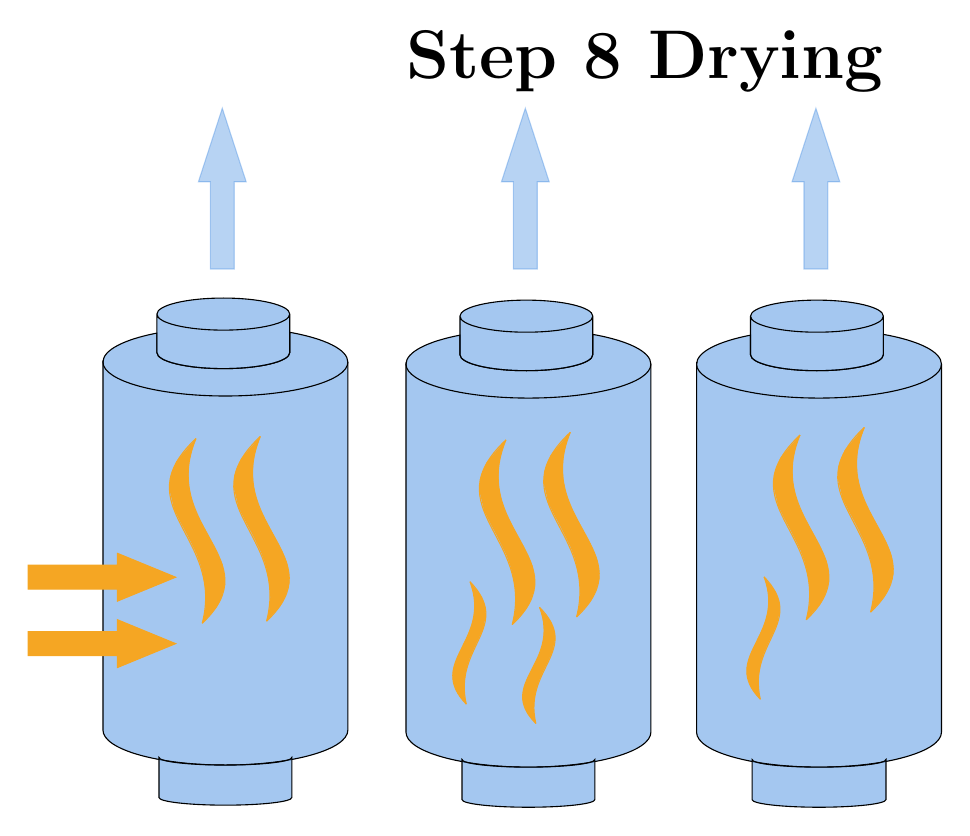
\begin{tikzpicture}[x=0.75pt,y=0.75pt,yscale=-1,xscale=1]
			%uncomment if require: \path (0,458); %set diagram left start at 0, and has height of 458
			
			%Shape: Path Data [id:dp8636157552152955] 
			\draw  [fill={rgb, 255:red, 74; green, 144; blue, 226 }  ,fill opacity=0.5 ] (305.5,343.14) .. controls (305.5,352.45) and (279.08,360) .. (246.5,360) .. controls (213.92,360) and (187.5,352.45) .. (187.5,343.14) -- (187.5,165.86) .. controls (187.5,160.04) and (197.81,154.91) .. (213.5,151.88) -- (213.5,161.27) .. controls (213.5,165.54) and (227.83,169) .. (245.5,169) .. controls (263.17,169) and (277.5,165.54) .. (277.5,161.27) -- (277.5,151.51) .. controls (294.3,154.48) and (305.5,159.8) .. (305.5,165.86) -- (305.5,343.14) -- cycle ;
			%Flowchart: Stored Data [id:dp676883836511693] 
			\draw  [fill={rgb, 255:red, 74; green, 144; blue, 226 }  ,fill opacity=0.5 ] (214.5,375.64) -- (214.5,356.32) .. controls (214.5,358.35) and (228.83,360) .. (246.5,360) .. controls (264.17,360) and (278.5,358.35) .. (278.5,356.32) -- (278.5,375.64) .. controls (278.5,377.67) and (264.17,379.32) .. (246.5,379.32) .. controls (228.83,379.32) and (214.5,377.67) .. (214.5,375.64) -- cycle ;
			%Shape: Path Data [id:dp9914978051443916] 
			\draw  [fill={rgb, 255:red, 74; green, 144; blue, 226 }  ,fill opacity=0.5 ] (451.5,344.14) .. controls (451.5,353.45) and (425.08,361) .. (392.5,361) .. controls (359.92,361) and (333.5,353.45) .. (333.5,344.14) -- (333.5,166.86) .. controls (333.5,161.04) and (343.81,155.91) .. (359.5,152.88) -- (359.5,162.27) .. controls (359.5,166.54) and (373.83,170) .. (391.5,170) .. controls (409.17,170) and (423.5,166.54) .. (423.5,162.27) -- (423.5,152.51) .. controls (440.3,155.48) and (451.5,160.8) .. (451.5,166.86) -- (451.5,344.14) -- cycle ;
			%Flowchart: Stored Data [id:dp7055206857460394] 
			\draw  [fill={rgb, 255:red, 74; green, 144; blue, 226 }  ,fill opacity=0.5 ] (360.5,376.64) -- (360.5,357.32) .. controls (360.5,359.35) and (374.83,361) .. (392.5,361) .. controls (410.17,361) and (424.5,359.35) .. (424.5,357.32) -- (424.5,376.64) .. controls (424.5,378.67) and (410.17,380.32) .. (392.5,380.32) .. controls (374.83,380.32) and (360.5,378.67) .. (360.5,376.64) -- cycle ;
			%Shape: Path Data [id:dp7581052878848111] 
			\draw  [fill={rgb, 255:red, 74; green, 144; blue, 226 }  ,fill opacity=0.5 ] (591.5,344.14) .. controls (591.5,353.45) and (565.08,361) .. (532.5,361) .. controls (499.92,361) and (473.5,353.45) .. (473.5,344.14) -- (473.5,166.86) .. controls (473.5,161.04) and (483.81,155.91) .. (499.5,152.88) -- (499.5,162.27) .. controls (499.5,166.54) and (513.83,170) .. (531.5,170) .. controls (549.17,170) and (563.5,166.54) .. (563.5,162.27) -- (563.5,152.51) .. controls (580.3,155.48) and (591.5,160.8) .. (591.5,166.86) -- (591.5,344.14) -- cycle ;
			%Flowchart: Stored Data [id:dp18658004198405542] 
			\draw  [fill={rgb, 255:red, 74; green, 144; blue, 226 }  ,fill opacity=0.5 ] (500.25,376.64) -- (500.25,357.32) .. controls (500.25,359.35) and (514.69,361) .. (532.5,361) .. controls (550.31,361) and (564.75,359.35) .. (564.75,357.32) -- (564.75,376.64) .. controls (564.75,378.67) and (550.31,380.32) .. (532.5,380.32) .. controls (514.69,380.32) and (500.25,378.67) .. (500.25,376.64) -- cycle ;
			%Up Arrow [id:dp7414740157371841] 
			\draw  [color={rgb, 255:red, 74; green, 144; blue, 226 }  ,draw opacity=0.4 ][fill={rgb, 255:red, 74; green, 144; blue, 226 }  ,fill opacity=0.4 ] (233.5,78.99) -- (245,43.57) -- (256.5,78.99) -- (250.75,78.99) -- (250.75,121) -- (239.25,121) -- (239.25,78.99) -- cycle ;
			%Shape: Polygon [id:ds40642945725486] 
			\draw  [draw opacity=0][fill={rgb, 255:red, 245; green, 166; blue, 35 }  ,fill opacity=1 ] (381.67,203.33) -- (380.07,207.83) -- (379.27,210.63) -- (378.27,215.23) -- (378.07,221.03) -- (378.27,226.23) -- (379.47,232.23) -- (381.27,237.83) -- (384.07,243.43) -- (387.07,249.03) -- (389.47,253.63) -- (392.07,258.63) -- (394.47,264.03) -- (395.47,269.23) -- (395.67,274.03) -- (393.87,279.83) -- (391.47,284.83) -- (388.87,287.63) -- (384.67,292.33) -- (386.07,286.43) -- (386.47,280.83) -- (386.07,275.03) -- (384.87,268.03) -- (383.87,264.23) -- (381.87,258.83) -- (379.27,253.43) -- (377.27,249.43) -- (374.07,243.43) -- (371.07,237.23) -- (368.87,227.83) -- (369.17,222.08) -- (372.27,214.23) -- cycle ;
			%Curve Lines [id:da2748166199730038] 
			\draw [color={rgb, 255:red, 245; green, 166; blue, 35 }  ,draw opacity=1 ]   (381.67,203.33) .. controls (363.67,246.33) and (417.67,261.33) .. (384.67,292.33) ;
			%Curve Lines [id:da9494211071025945] 
			\draw [color={rgb, 255:red, 245; green, 166; blue, 35 }  ,draw opacity=1 ]   (381.67,203.33) .. controls (346.67,236.33) and (395.67,250.33) .. (384.67,292.33) ;
			
			
			%Shape: Polygon [id:ds4673870177314182] 
			\draw  [draw opacity=0][fill={rgb, 255:red, 245; green, 166; blue, 35 }  ,fill opacity=1 ] (412.67,199.67) -- (411.07,204.17) -- (410.27,206.97) -- (409.27,211.57) -- (409.07,217.37) -- (409.27,222.57) -- (410.47,228.57) -- (412.27,234.17) -- (415.07,239.77) -- (418.07,245.37) -- (420.47,249.97) -- (423.07,254.97) -- (425.47,260.37) -- (426.47,265.57) -- (426.67,270.37) -- (424.87,276.17) -- (422.47,281.17) -- (419.87,283.97) -- (415.67,288.67) -- (417.07,282.77) -- (417.47,277.17) -- (417.07,271.37) -- (415.87,264.37) -- (414.87,260.57) -- (412.87,255.17) -- (410.27,249.77) -- (408.27,245.77) -- (405.07,239.77) -- (402.07,233.57) -- (399.87,224.17) -- (400.17,218.42) -- (403.27,210.57) -- cycle ;
			%Curve Lines [id:da06518814973284248] 
			\draw [color={rgb, 255:red, 245; green, 166; blue, 35 }  ,draw opacity=1 ]   (412.67,199.67) .. controls (394.67,242.67) and (448.67,257.67) .. (415.67,288.67) ;
			%Curve Lines [id:da9293762817201134] 
			\draw [color={rgb, 255:red, 245; green, 166; blue, 35 }  ,draw opacity=1 ]   (412.67,199.67) .. controls (377.67,232.67) and (426.67,246.67) .. (415.67,288.67) ;
			
			
			%Shape: Polygon [id:ds20107559469399994] 
			\draw  [draw opacity=0][fill={rgb, 255:red, 245; green, 166; blue, 35 }  ,fill opacity=1 ] (364.35,271.67) -- (365.31,274.65) -- (365.79,276.51) -- (366.38,279.56) -- (366.5,283.4) -- (366.38,286.85) -- (365.67,290.83) -- (364.59,294.54) -- (362.92,298.25) -- (361.13,301.96) -- (359.7,305.01) -- (358.15,308.33) -- (356.72,311.91) -- (356.12,315.35) -- (356,318.54) -- (357.07,322.38) -- (358.51,325.69) -- (360.06,327.55) -- (362.56,330.67) -- (361.73,326.76) -- (361.49,323.04) -- (361.73,319.2) -- (362.44,314.56) -- (363.04,312.04) -- (364.23,308.46) -- (365.79,304.88) -- (366.98,302.23) -- (368.89,298.25) -- (370.68,294.14) -- (371.99,287.91) -- (371.81,284.1) -- (369.96,278.89) -- cycle ;
			%Curve Lines [id:da9770296442665731] 
			\draw [color={rgb, 255:red, 245; green, 166; blue, 35 }  ,draw opacity=1 ]   (364.35,271.67) .. controls (375.09,300.17) and (342.87,310.12) .. (362.56,330.67) ;
			%Curve Lines [id:da7682345246406161] 
			\draw [color={rgb, 255:red, 245; green, 166; blue, 35 }  ,draw opacity=1 ]   (364.35,271.67) .. controls (385.24,293.54) and (356,302.82) .. (362.56,330.67) ;
			
			
			%Shape: Polygon [id:ds5586749920092644] 
			\draw  [draw opacity=0][fill={rgb, 255:red, 245; green, 166; blue, 35 }  ,fill opacity=1 ] (397.85,284) -- (398.78,286.83) -- (399.25,288.59) -- (399.83,291.49) -- (399.95,295.14) -- (399.83,298.41) -- (399.13,302.18) -- (398.08,305.71) -- (396.44,309.23) -- (394.69,312.76) -- (393.29,315.65) -- (391.77,318.8) -- (390.37,322.19) -- (389.78,325.47) -- (389.67,328.49) -- (390.72,332.13) -- (392.12,335.28) -- (393.64,337.04) -- (396.09,340) -- (395.28,336.29) -- (395.04,332.76) -- (395.28,329.11) -- (395.98,324.71) -- (396.56,322.32) -- (397.73,318.92) -- (399.25,315.52) -- (400.42,313.01) -- (402.29,309.23) -- (404.04,305.33) -- (405.33,299.42) -- (405.15,295.8) -- (403.34,290.86) -- cycle ;
			%Curve Lines [id:da5875371999359253] 
			\draw [color={rgb, 255:red, 245; green, 166; blue, 35 }  ,draw opacity=1 ]   (397.85,284) .. controls (408.36,311.06) and (376.81,320.49) .. (396.09,340) ;
			%Curve Lines [id:da3048303725522802] 
			\draw [color={rgb, 255:red, 245; green, 166; blue, 35 }  ,draw opacity=1 ]   (397.85,284) .. controls (418.3,304.76) and (389.67,313.57) .. (396.09,340) ;
			
			
			%Up Arrow [id:dp40478803296430965] 
			\draw  [color={rgb, 255:red, 245; green, 166; blue, 35 }  ,draw opacity=1 ][fill={rgb, 255:red, 245; green, 166; blue, 35 }  ,fill opacity=1 ] (194.5,258) -- (222.5,269.5) -- (194.5,281) -- (194.5,275.25) -- (151.5,275.25) -- (151.5,263.75) -- (194.5,263.75) -- cycle ;
			%Up Arrow [id:dp26025828941126183] 
			\draw  [color={rgb, 255:red, 245; green, 166; blue, 35 }  ,draw opacity=1 ][fill={rgb, 255:red, 245; green, 166; blue, 35 }  ,fill opacity=1 ] (194.5,290) -- (222.5,301.5) -- (194.5,313) -- (194.5,307.25) -- (151.5,307.25) -- (151.5,295.75) -- (194.5,295.75) -- cycle ;
			%Shape: Polygon [id:ds3223925852663938] 
			\draw  [draw opacity=0][fill={rgb, 255:red, 245; green, 166; blue, 35 }  ,fill opacity=1 ] (232.33,202.67) -- (230.73,207.17) -- (229.93,209.97) -- (228.93,214.57) -- (228.73,220.37) -- (228.93,225.57) -- (230.13,231.57) -- (231.93,237.17) -- (234.73,242.77) -- (237.73,248.37) -- (240.13,252.97) -- (242.73,257.97) -- (245.13,263.37) -- (246.13,268.57) -- (246.33,273.37) -- (244.53,279.17) -- (242.13,284.17) -- (239.53,286.97) -- (235.33,291.67) -- (236.73,285.77) -- (237.13,280.17) -- (236.73,274.37) -- (235.53,267.37) -- (234.53,263.57) -- (232.53,258.17) -- (229.93,252.77) -- (227.93,248.77) -- (224.73,242.77) -- (221.73,236.57) -- (219.53,227.17) -- (219.83,221.42) -- (222.93,213.57) -- cycle ;
			%Curve Lines [id:da6528284989344888] 
			\draw [color={rgb, 255:red, 245; green, 166; blue, 35 }  ,draw opacity=1 ]   (232.33,202.67) .. controls (214.33,245.67) and (268.33,260.67) .. (235.33,291.67) ;
			%Curve Lines [id:da6670801432183355] 
			\draw [color={rgb, 255:red, 245; green, 166; blue, 35 }  ,draw opacity=1 ]   (232.33,202.67) .. controls (197.33,235.67) and (246.33,249.67) .. (235.33,291.67) ;
			
			
			%Shape: Polygon [id:ds2937791440055918] 
			\draw  [draw opacity=0][fill={rgb, 255:red, 245; green, 166; blue, 35 }  ,fill opacity=1 ] (263.33,201.67) -- (261.73,206.17) -- (260.93,208.97) -- (259.93,213.57) -- (259.73,219.37) -- (259.93,224.57) -- (261.13,230.57) -- (262.93,236.17) -- (265.73,241.77) -- (268.73,247.37) -- (271.13,251.97) -- (273.73,256.97) -- (276.13,262.37) -- (277.13,267.57) -- (277.33,272.37) -- (275.53,278.17) -- (273.13,283.17) -- (270.53,285.97) -- (266.33,290.67) -- (267.73,284.77) -- (268.13,279.17) -- (267.73,273.37) -- (266.53,266.37) -- (265.53,262.57) -- (263.53,257.17) -- (260.93,251.77) -- (258.93,247.77) -- (255.73,241.77) -- (252.73,235.57) -- (250.53,226.17) -- (250.83,220.42) -- (253.93,212.57) -- cycle ;
			%Curve Lines [id:da36776234934459884] 
			\draw [color={rgb, 255:red, 245; green, 166; blue, 35 }  ,draw opacity=1 ]   (263.33,201.67) .. controls (245.33,244.67) and (299.33,259.67) .. (266.33,290.67) ;
			%Curve Lines [id:da7810393140360538] 
			\draw [color={rgb, 255:red, 245; green, 166; blue, 35 }  ,draw opacity=1 ]   (263.33,201.67) .. controls (228.33,234.67) and (277.33,248.67) .. (266.33,290.67) ;
			
			
			%Shape: Polygon [id:ds4971230584725458] 
			\draw  [draw opacity=0][fill={rgb, 255:red, 245; green, 166; blue, 35 }  ,fill opacity=1 ] (523.33,201) -- (521.73,205.5) -- (520.93,208.3) -- (519.93,212.9) -- (519.73,218.7) -- (519.93,223.9) -- (521.13,229.9) -- (522.93,235.5) -- (525.73,241.1) -- (528.73,246.7) -- (531.13,251.3) -- (533.73,256.3) -- (536.13,261.7) -- (537.13,266.9) -- (537.33,271.7) -- (535.53,277.5) -- (533.13,282.5) -- (530.53,285.3) -- (526.33,290) -- (527.73,284.1) -- (528.13,278.5) -- (527.73,272.7) -- (526.53,265.7) -- (525.53,261.9) -- (523.53,256.5) -- (520.93,251.1) -- (518.93,247.1) -- (515.73,241.1) -- (512.73,234.9) -- (510.53,225.5) -- (510.83,219.75) -- (513.93,211.9) -- cycle ;
			%Curve Lines [id:da33907491162061165] 
			\draw [color={rgb, 255:red, 245; green, 166; blue, 35 }  ,draw opacity=1 ]   (523.33,201) .. controls (505.33,244) and (559.33,259) .. (526.33,290) ;
			%Curve Lines [id:da6670755528046683] 
			\draw [color={rgb, 255:red, 245; green, 166; blue, 35 }  ,draw opacity=1 ]   (523.33,201) .. controls (488.33,234) and (537.33,248) .. (526.33,290) ;
			
			
			%Shape: Polygon [id:ds1623984812913849] 
			\draw  [draw opacity=0][fill={rgb, 255:red, 245; green, 166; blue, 35 }  ,fill opacity=1 ] (554.33,197.33) -- (552.73,201.83) -- (551.93,204.63) -- (550.93,209.23) -- (550.73,215.03) -- (550.93,220.23) -- (552.13,226.23) -- (553.93,231.83) -- (556.73,237.43) -- (559.73,243.03) -- (562.13,247.63) -- (564.73,252.63) -- (567.13,258.03) -- (568.13,263.23) -- (568.33,268.03) -- (566.53,273.83) -- (564.13,278.83) -- (561.53,281.63) -- (557.33,286.33) -- (558.73,280.43) -- (559.13,274.83) -- (558.73,269.03) -- (557.53,262.03) -- (556.53,258.23) -- (554.53,252.83) -- (551.93,247.43) -- (549.93,243.43) -- (546.73,237.43) -- (543.73,231.23) -- (541.53,221.83) -- (541.83,216.08) -- (544.93,208.23) -- cycle ;
			%Curve Lines [id:da3902524320518824] 
			\draw [color={rgb, 255:red, 245; green, 166; blue, 35 }  ,draw opacity=1 ]   (554.33,197.33) .. controls (536.33,240.33) and (590.33,255.33) .. (557.33,286.33) ;
			%Curve Lines [id:da013274374700474545] 
			\draw [color={rgb, 255:red, 245; green, 166; blue, 35 }  ,draw opacity=1 ]   (554.33,197.33) .. controls (519.33,230.33) and (568.33,244.33) .. (557.33,286.33) ;
			
			
			%Shape: Polygon [id:ds5391402732435858] 
			\draw  [draw opacity=0][fill={rgb, 255:red, 245; green, 166; blue, 35 }  ,fill opacity=1 ] (506.02,269.33) -- (506.98,272.32) -- (507.45,274.17) -- (508.05,277.22) -- (508.17,281.07) -- (508.05,284.51) -- (507.33,288.49) -- (506.26,292.2) -- (504.59,295.92) -- (502.8,299.63) -- (501.37,302.68) -- (499.81,305.99) -- (498.38,309.57) -- (497.79,313.02) -- (497.67,316.2) -- (498.74,320.05) -- (500.17,323.36) -- (501.72,325.22) -- (504.23,328.33) -- (503.4,324.42) -- (503.16,320.71) -- (503.4,316.86) -- (504.11,312.22) -- (504.71,309.71) -- (505.9,306.13) -- (507.45,302.55) -- (508.65,299.89) -- (510.56,295.92) -- (512.35,291.81) -- (513.66,285.57) -- (513.48,281.76) -- (511.63,276.56) -- cycle ;
			%Curve Lines [id:da348959127377361] 
			\draw [color={rgb, 255:red, 245; green, 166; blue, 35 }  ,draw opacity=1 ]   (506.02,269.33) .. controls (516.76,297.84) and (484.54,307.78) .. (504.23,328.33) ;
			%Curve Lines [id:da7567572707254564] 
			\draw [color={rgb, 255:red, 245; green, 166; blue, 35 }  ,draw opacity=1 ]   (506.02,269.33) .. controls (526.91,291.21) and (497.67,300.49) .. (504.23,328.33) ;
			
			
			%Shape: Can [id:dp8395558193343627] 
			\draw  [fill={rgb, 255:red, 74; green, 144; blue, 226 }  ,fill opacity=0.5 ] (563.5,143.73) -- (563.5,162.27) .. controls (563.5,166.54) and (549.17,170) .. (531.5,170) .. controls (513.83,170) and (499.5,166.54) .. (499.5,162.27) -- (499.5,143.73) .. controls (499.5,139.46) and (513.83,136) .. (531.5,136) .. controls (549.17,136) and (563.5,139.46) .. (563.5,143.73) .. controls (563.5,147.99) and (549.17,151.45) .. (531.5,151.45) .. controls (513.83,151.45) and (499.5,147.99) .. (499.5,143.73) ;
			%Shape: Arc [id:dp38927215246150704] 
			\draw  [draw opacity=0] (591.5,166.86) .. controls (591.5,175.88) and (565.08,183.19) .. (532.5,183.19) .. controls (499.92,183.19) and (473.5,175.88) .. (473.5,166.86) .. controls (473.5,166.49) and (473.54,166.13) .. (473.63,165.78) -- (532.5,166.86) -- cycle ; \draw   (591.5,166.86) .. controls (591.5,175.88) and (565.08,183.19) .. (532.5,183.19) .. controls (499.92,183.19) and (473.5,175.88) .. (473.5,166.86) .. controls (473.5,166.49) and (473.54,166.13) .. (473.63,165.78) ;  
			%Shape: Can [id:dp6937495778315892] 
			\draw  [fill={rgb, 255:red, 74; green, 144; blue, 226 }  ,fill opacity=0.5 ] (423.5,143.73) -- (423.5,162.27) .. controls (423.5,166.54) and (409.17,170) .. (391.5,170) .. controls (373.83,170) and (359.5,166.54) .. (359.5,162.27) -- (359.5,143.73) .. controls (359.5,139.46) and (373.83,136) .. (391.5,136) .. controls (409.17,136) and (423.5,139.46) .. (423.5,143.73) .. controls (423.5,147.99) and (409.17,151.45) .. (391.5,151.45) .. controls (373.83,151.45) and (359.5,147.99) .. (359.5,143.73) ;
			%Shape: Arc [id:dp07565595692588256] 
			\draw  [draw opacity=0] (451.5,166.86) .. controls (451.5,175.88) and (425.08,183.19) .. (392.5,183.19) .. controls (359.92,183.19) and (333.5,175.88) .. (333.5,166.86) .. controls (333.5,166.49) and (333.54,166.13) .. (333.63,165.78) -- (392.5,166.86) -- cycle ; \draw   (451.5,166.86) .. controls (451.5,175.88) and (425.08,183.19) .. (392.5,183.19) .. controls (359.92,183.19) and (333.5,175.88) .. (333.5,166.86) .. controls (333.5,166.49) and (333.54,166.13) .. (333.63,165.78) ;  
			%Shape: Can [id:dp16020242495345627] 
			\draw  [fill={rgb, 255:red, 74; green, 144; blue, 226 }  ,fill opacity=0.5 ] (277.5,142.73) -- (277.5,161.27) .. controls (277.5,165.54) and (263.17,169) .. (245.5,169) .. controls (227.83,169) and (213.5,165.54) .. (213.5,161.27) -- (213.5,142.73) .. controls (213.5,138.46) and (227.83,135) .. (245.5,135) .. controls (263.17,135) and (277.5,138.46) .. (277.5,142.73) .. controls (277.5,146.99) and (263.17,150.45) .. (245.5,150.45) .. controls (227.83,150.45) and (213.5,146.99) .. (213.5,142.73) ;
			%Shape: Arc [id:dp655095418341306] 
			\draw  [draw opacity=0] (305.5,165.86) .. controls (305.5,174.88) and (279.08,182.19) .. (246.5,182.19) .. controls (213.92,182.19) and (187.5,174.88) .. (187.5,165.86) .. controls (187.5,165.49) and (187.54,165.13) .. (187.63,164.78) -- (246.5,165.86) -- cycle ; \draw   (305.5,165.86) .. controls (305.5,174.88) and (279.08,182.19) .. (246.5,182.19) .. controls (213.92,182.19) and (187.5,174.88) .. (187.5,165.86) .. controls (187.5,165.49) and (187.54,165.13) .. (187.63,164.78) ;  
			%Up Arrow [id:dp2787721508361427] 
			\draw  [color={rgb, 255:red, 74; green, 144; blue, 226 }  ,draw opacity=0.4 ][fill={rgb, 255:red, 74; green, 144; blue, 226 }  ,fill opacity=0.4 ] (379.5,78.99) -- (391,43.57) -- (402.5,78.99) -- (396.75,78.99) -- (396.75,121) -- (385.25,121) -- (385.25,78.99) -- cycle ;
			%Up Arrow [id:dp5799576746273714] 
			\draw  [color={rgb, 255:red, 74; green, 144; blue, 226 }  ,draw opacity=0.4 ][fill={rgb, 255:red, 74; green, 144; blue, 226 }  ,fill opacity=0.4 ] (519.5,78.99) -- (531,43.57) -- (542.5,78.99) -- (536.75,78.99) -- (536.75,121) -- (525.25,121) -- (525.25,78.99) -- cycle ;
			
			% Text Node
			\draw (332.33,5) node [anchor=north west][inner sep=0.75pt]  [font=\fontsize{30pt}{36pt}\selectfont] [align=left] {\textbf{Step 8 Drying}};		\end{tikzpicture}
	    \vspace{6pt}
\end{minipage}}
		\end{center}
	\end{aaaa}
\end{document}